\chapter{Introducción}

Este Trabajo de Fin de Grado consiste en desarrollar un módulo
software que registre automáticamente información sobre
la recolección de cultivos leñosos haciendo uso de un
sistema de control embebido.

Este proyecto es software libre, y está liberado con
la licencia \textbf{GNU Affero General Public License} \cite{agplv3}.

\section{Motivación}

En España existen 23.848.757 hectáreas de superficie agrícola utilizada%
\footnote{%
Según el INE, conjunto de la superficie de tierras labradas y tierras
para pastos permanentes.
}%
al aire libre, de las cuales \textbf{4.657.182 hectáreas se dedican a cultivos leñosos}
 \cite{INEdistribucionDeLaSuperficiePorTamaño}.
Entre estos predominan el cultivo del olivar, del viñedo, de los cítricos,
de los frutos secos como las almendras o los pistachos y otros frutales
 \cite{INEpanoramicaCensoAgrario}.

\begin{figure}[!b]
    \centering
    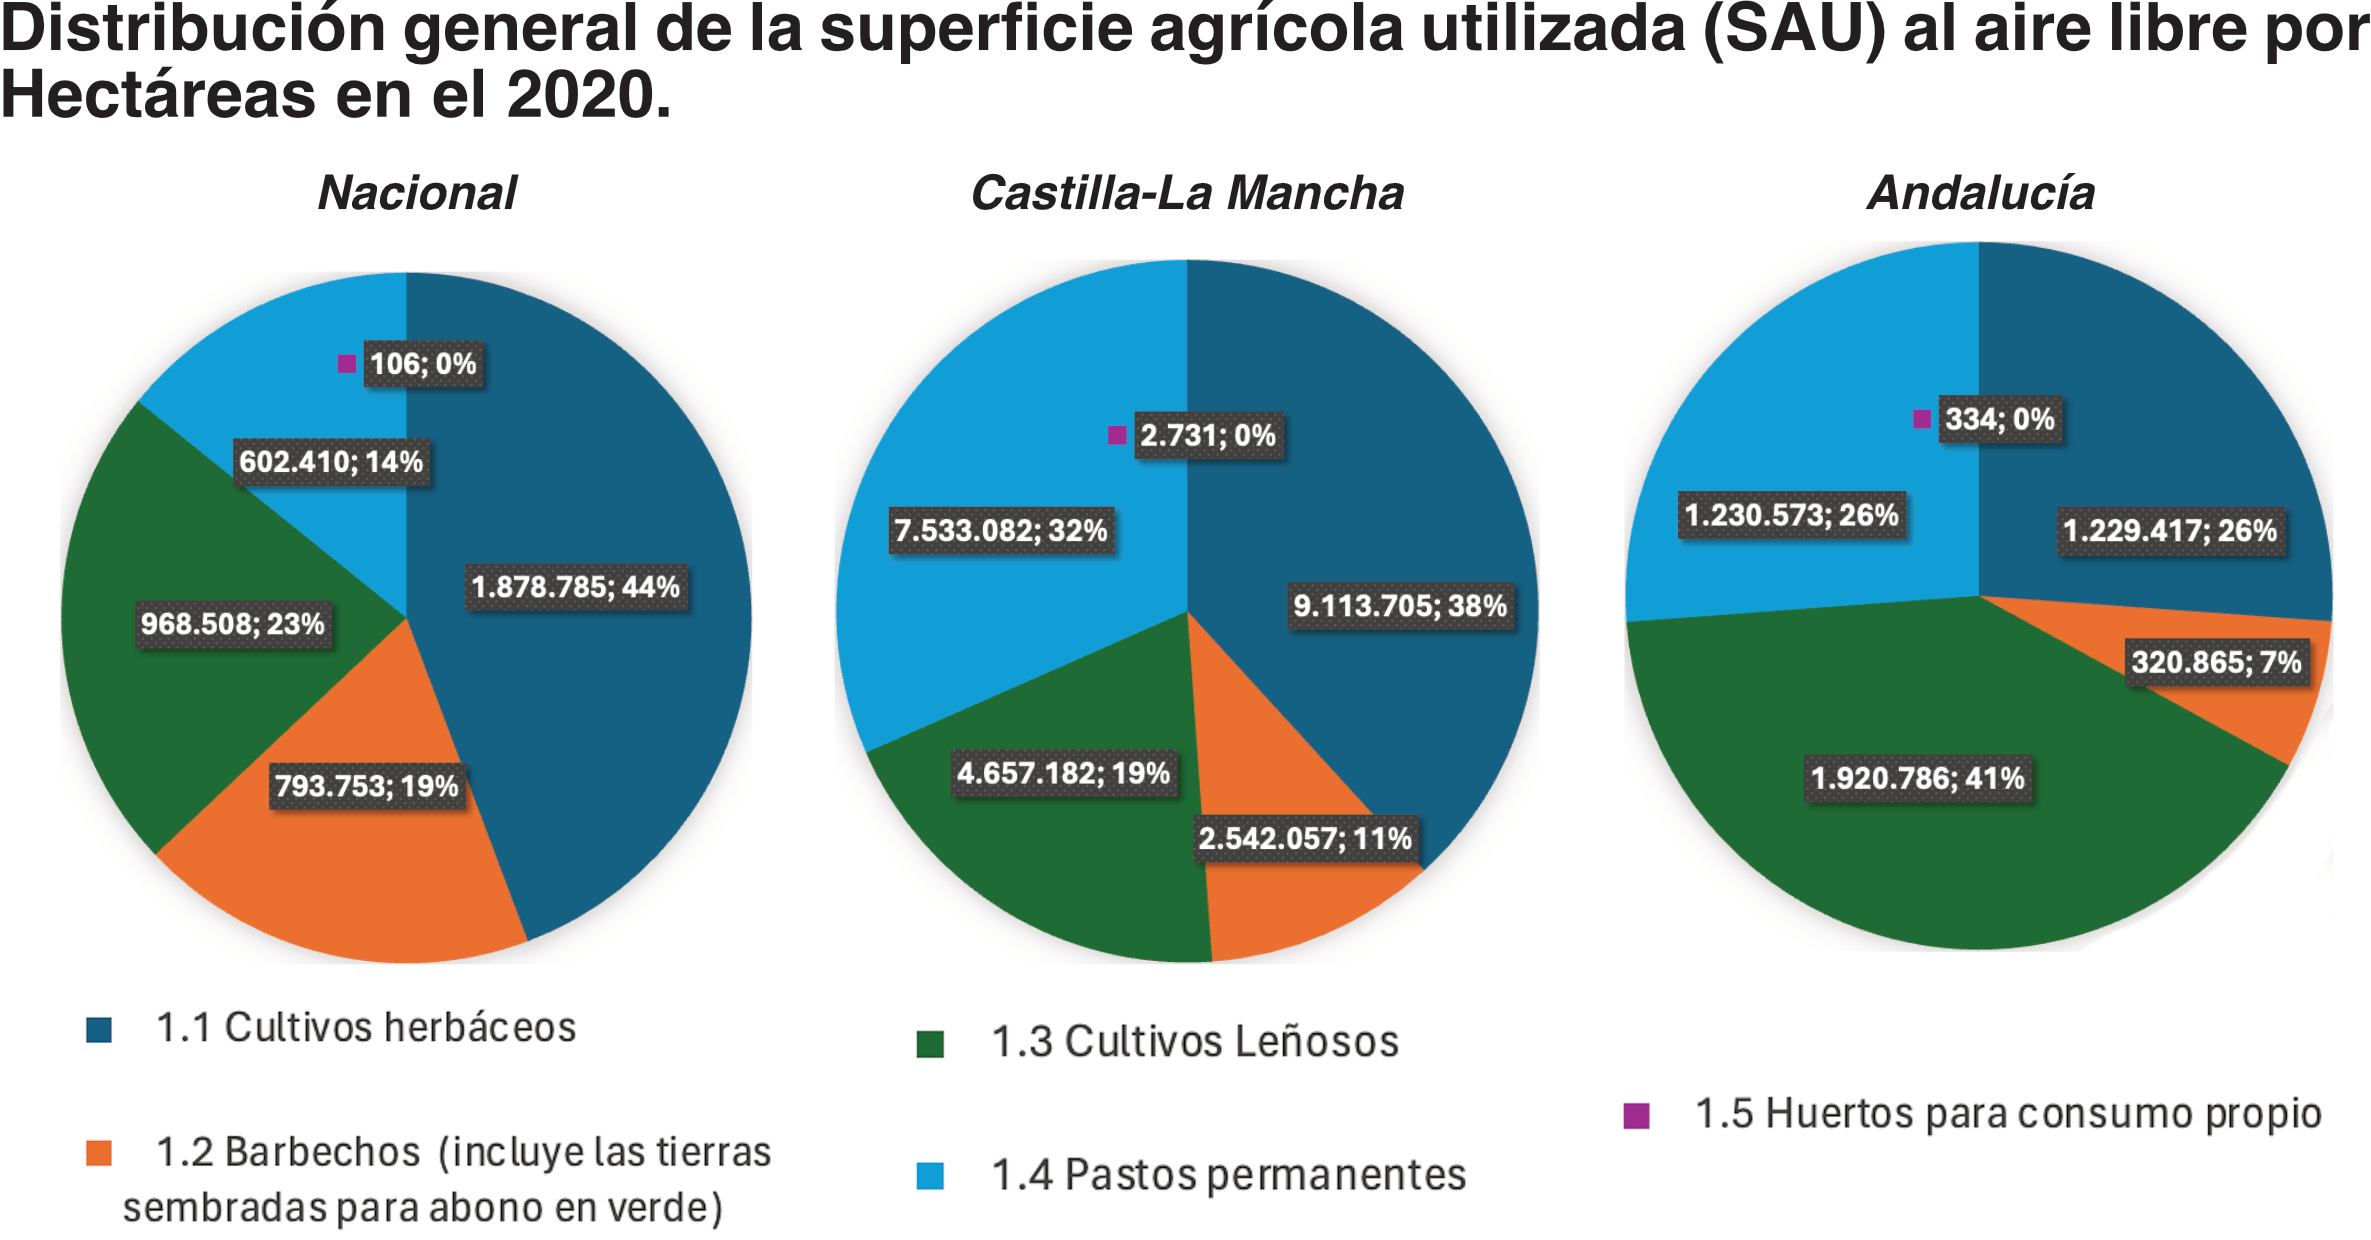
\includegraphics[width=\textwidth]{distribucion-SAU-segun-cultivo-aire-libre.png}
    \caption{\textit{Distribución general de la SAU al aire libre por hectáreas
    según \cite{INEdistribucionDeLaSuperficiePorTamaño}. Los territorios de Andalucía y Castilla-La Mancha
    acumulan aproximadamente el 62\% de los cultivos leñosos en territorio nacional.
    Elaboración propia.}}
\end{figure}

\subsection{Situación de las explotaciones agrícolas en España}

\textbf{La explotación} de la superficie agrícola utilizada \textbf{se realiza mayoritariamente por personas
físicas}. Aunque \textbf{observamos un mayor número de sociedades mercantiles
a medida que aumenta el tamaño de explotación}, la proporción de estas no llega a más del 30\%
con respecto a las personas físicas, y este porcentaje sólo se da en latifundios\footnote{%
    Consideramos que una explotación agrícola es un latifundio a partir de las 100 hectáreas.
}%
.
 \cite[Personalidad jurídica según el tamaño de explotación]{INEpanoramicaCensoAgrario}.

Además, \textbf{no existe apenas una renovación de los jefes de explotación}%
\footnote{%
    Según Eustat, la persona física responsable de las actividades financieras y de producción, corrientes y cotidianas de una explotación agrícola.
}%
. Según el INE, no hay comarca en la que menos del 60\% de los jefes de explotación tenga más de 45 años.
Y de entre todos los jefes de explotación no hay comarca que tenga más de un 25\% de estos con formación
reglada específica, \textbf{llegando a menos del 2,84\% regiones en las que predominan los cultivos leñosos}
 \cite[Formación de los jefes de explotación]{INEpanoramicaCensoAgrario}.

\subsection{Gestión de las explotaciones de cultivos leñosos}

\begin{figure}[!b]
    \centering
    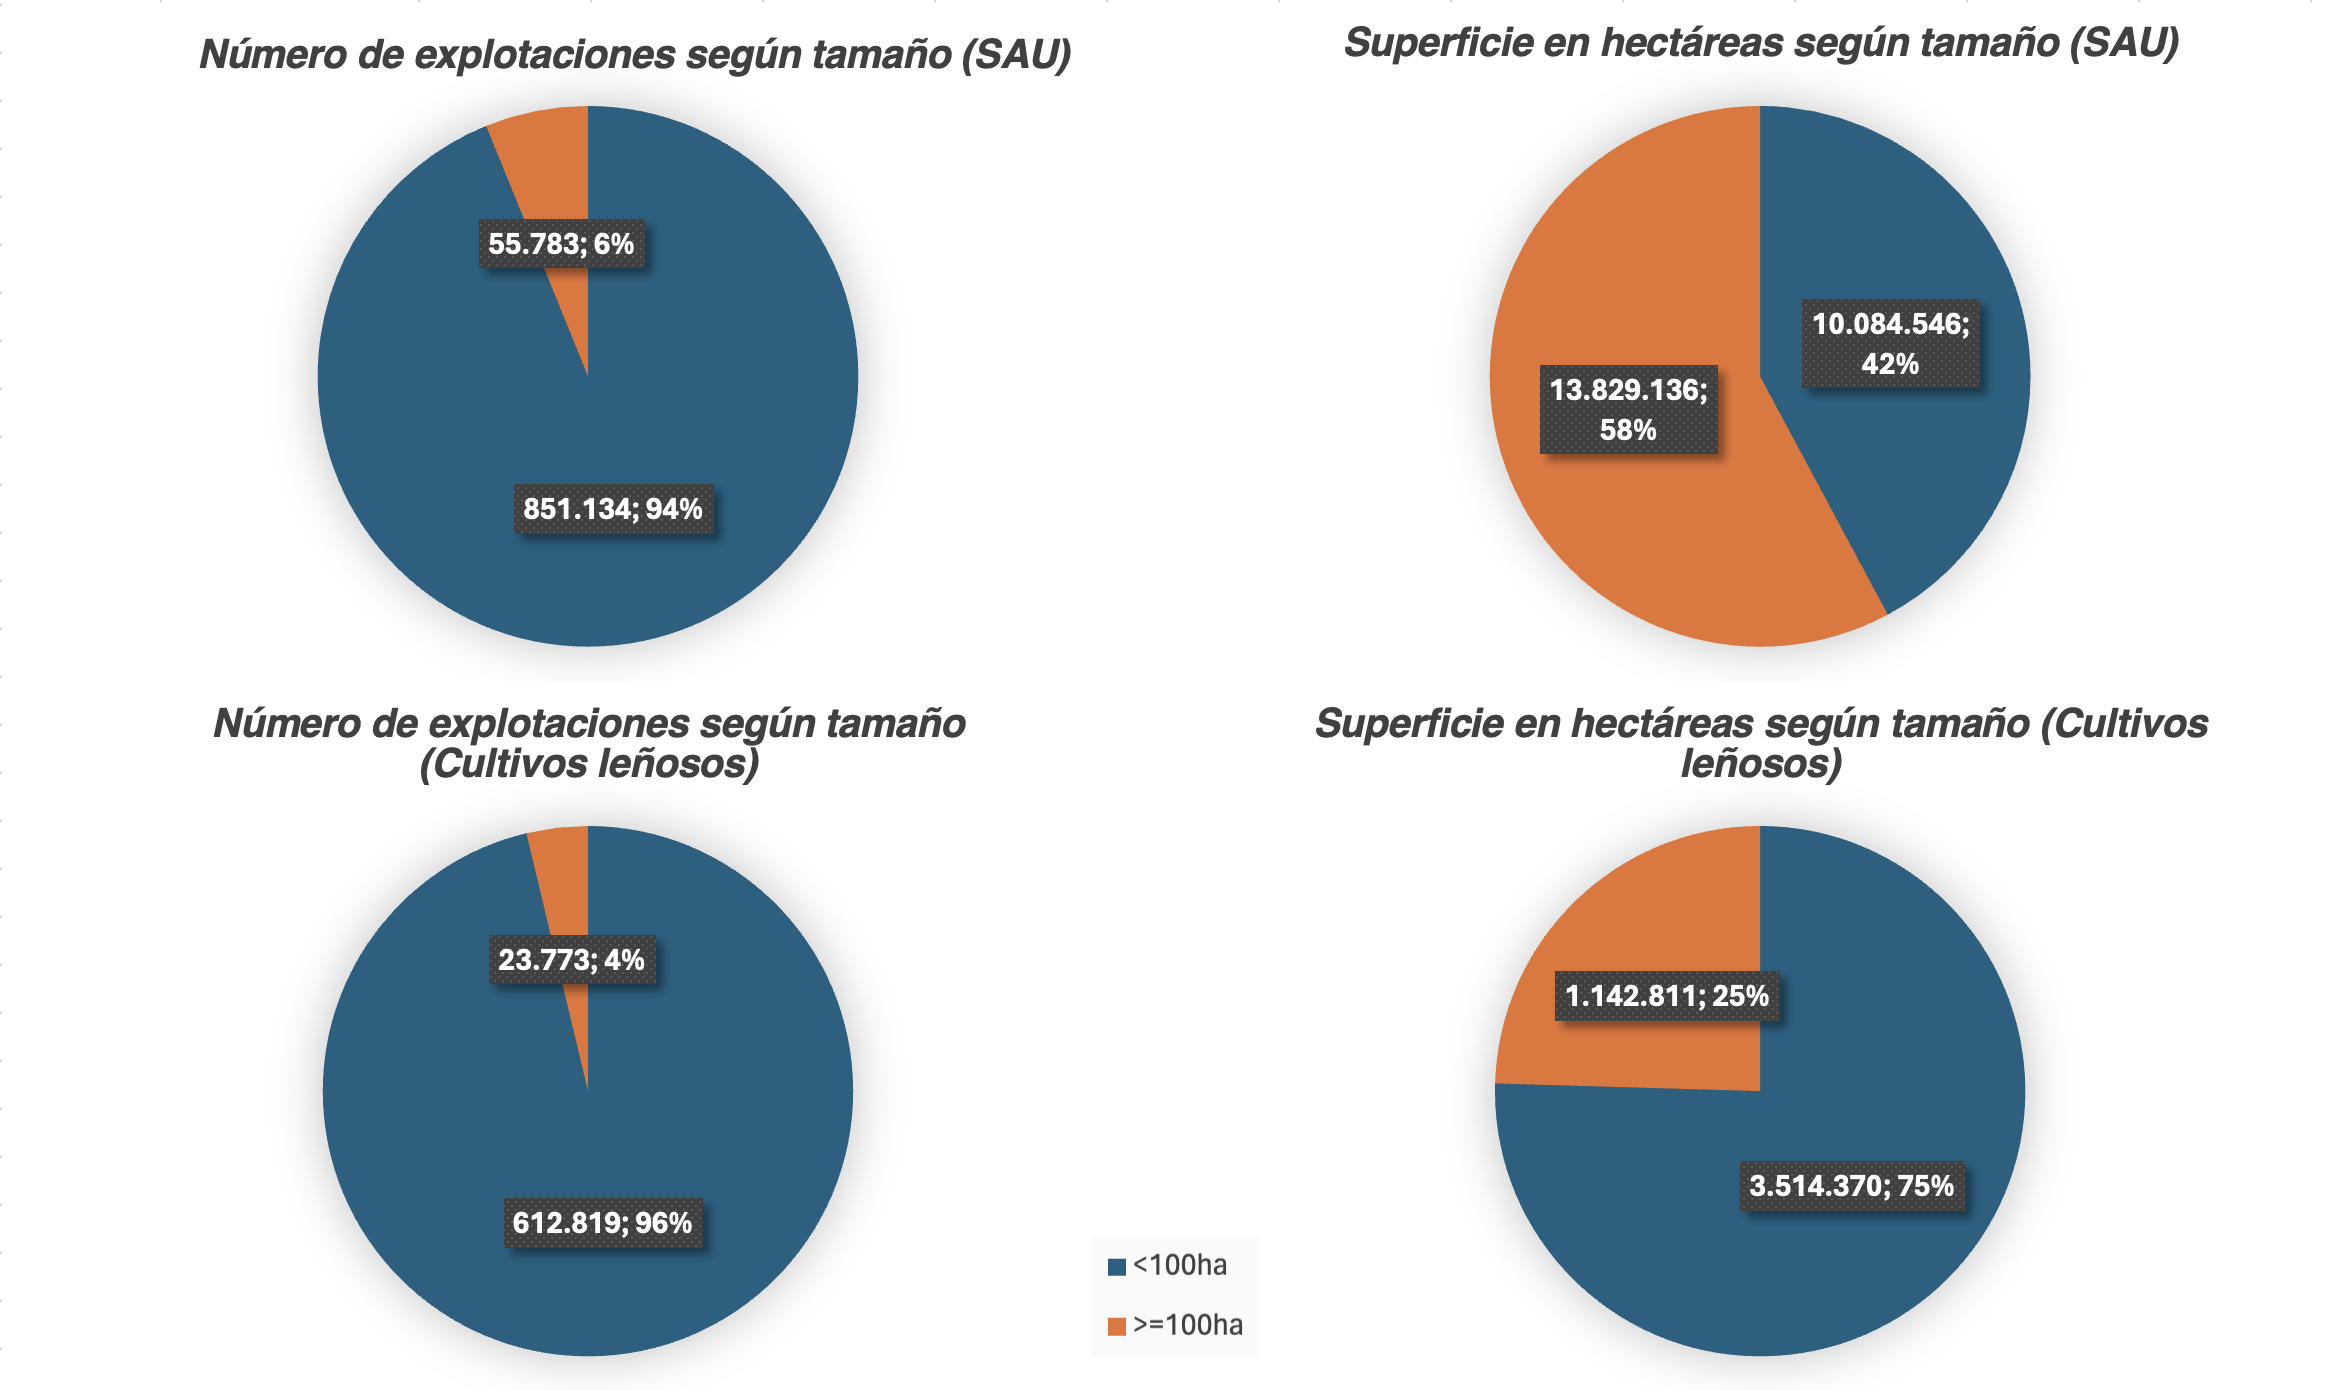
\includegraphics[width=\textwidth]{distribucion-SAU-segun-tamaño.png}
    \caption{\textit{Distribución general de la SAU por tamaño de la explotación según
    \cite{INEdistribucionDeLaSuperficiePorTamaño}. Apreciamos que, aunque es similar la
    proporción del número de explotaciones según el tamaño para la media de todos los tipos
    de cultivos y para los leñosos, la superficie ocupada para ambas categorías difiere
    significativamente. Elaboración propia.}}
\end{figure}

La geografía de este tipo de cultivos se concentra en Andalucía, Castilla-La Mancha y Extremadura.
 \cite[Reparto de la superficie dedicada a los grandes cultivos.]{INEpanoramicaCensoAgrario}

\textbf{Dos terceras partes del coste} de este tipo de cultivos \textbf{se destinan a la
recolección y a la poda}
 \cite{Mecaolivar}.
Entre las soluciones mecanizadas para la recolección encontramos principalmente
los vareadores eléctricos y los paraguas vibradores,
mientras que para la poda las tijeras eléctricas, las motosierras y
las trituradoras para motocultores.

Cada vez es menos rentable cultivar. La inversión en maquinaria y mecanización
busca prescindir de la mayor mano de obra posible.

Además, algunos jefes de explotación deciden externalizar la recolección
de sus cultivos a empresas especializadas.

\section{Problema a resolver} \label{sec:problema_a_resolver}

\textbf{Buscamos describir de una forma clara y concisa el problema y sus
circunstancias}. Consideramos que el problema se describe de forma clara y
concisa cuando se enuncia con el mínimo nivel de complejidad posible%
%
\footnote{Aunque
no por ello debe ser insuficiente. Un mito extendido acerca de las metodologías ágiles
es que no necesitamos tener una idea clara del problema antes de empezar a desarrollar
una solución. Nada mas lejos de la verdad, lo que se busca con los métodos ágiles en la
fase de análisis es poner a prueba empíricamente que nuestro modelo del problema es fiel
a la realidad, y que el problema que estamos resolviendo es el correcto antes de proponer
una solución arquitectónica. Así se concibe en las publicaciones que iniciaron el hoy
degenerado movimiento. \cite{AgileBackToBasics}
}%
, el lenguaje que se utiliza es simple pero adecuado
en su contexto y no tiene sesgos hacia ninguna solución.

Nuestro cliente acude a nosotros para desarrollar una solución propia de
estadísticas de recolección en cultivos leñosos.

Existen empresas y trabajadores los cuales, a cambio de dinero, trabajan la
tierra de un tercero con su maquinaria.

\textbf{Quien contrata el servicio} quiere reportes/resúmenes acerca de la actividad
de la máquina dado un intervalo de tiempo. Quiere conocer, a partir de una fecha y hora de inicio y otra de final:

\begin{enumerate}[noitemsep,nolistsep]
   \item Tiempo medio entre vibraciones.
   \item Tiempo medio vibrando.
   \item Posición de los árboles vibrados.
   \item Tiempo de trabajo efectivo.
\end{enumerate}

\textbf{Tanto quien contrata el servicio como quien lo ejecuta} quieren poder consultar
los datos sin necesidad de conexión a Internet y quieren poder comprobar la veracidad de los datos.

\section{Objetivo}

Con este proyecto \textbf{queremos obtener un producto que genere informes
de trabajo de un paraguas vibrador}, de forma que permita tanto a
quien recolecta el fruto como al jefe de explotación tener información
acerca de una jornada de trabajo para certificar el trabajo realizado.

Concretamente, según vemos en la sección del problema a resolver,
buscamos \textbf{desarrollar
una solución software que permita registrar y visualizar
información sobre la recolección de cultivos
leñosos con paraguas vibradores según los criterios de nuestro cliente},
con la restricción de que el registro y el exportado pueda ejecutarse en
una plataforma hardware ya distribuida en el mercado.

\vspace*{\fill}

\section{Estructura del documento}

Después de distintas iteraciones a lo largo del desarrollo de este Trabajo de Fin de Grado
llegamos a la división de la memoria en los siguientes capítulos.

\begin{enumerate}
    \item \textbf{Introducción.} Donde exponemos el problema a resolver,
          sus circunstancias actuales y los objetivos que se quieren alcanzar en rasgos generales.

    \item \textbf{Metodología.} Donde exponemos cómo abordamos el desarrollo del problema y su solución y por qué.
          Explicamos qué metodología seguimos, cómo estimamos el tiempo y los costes, cómo seguimos el progreso
          del proyecto y cómo registramos métricas para los objetivos del sexto capítulo de esta memoria.

    \item \textbf{Análisis de requisitos.} Donde decidimos en una primera aproximación cómo debe comportarse el
          sistema, de forma que evitamos construir un PMV\footnote{\textit{Producto Mínimamente Viable}.
          Es un producto cuyo objetivo es obtener realimentación de los usuarios antes de realizar un diseño de
          un producto para el cuál desconocemos la cabida que va a tener.} incorrecto.

    \item \textbf{Implementación.} Donde describimos cómo llevamos a cabo el desarrollo software
          de la solución propuesta.

    \item \textbf{Conclusión.} Donde realizamos una visita crítica a las ideas de los puntos
          anteriores una vez finalizado el proyecto y exponemos nuevas ideas surgidas de la experiencia.
\end{enumerate}
